Ya sabemos usar LaTeX, crear documentos complejos, presentaciones y
hasta macros propias. Este capítulo es un poco diferente a los
anteriores ya que en lugar de averiguar cómo se hacen las cosas en
LaTeX, vamos a hablar de herramientas externas y trucos que nos pueden
ayudar a la hora de crear nuestro documento.

Veremos algunos paquetes que simplifican el proceso de probar el
formato, cómo crear una plantilla o un registro de cambios y algunas
herramientas que no pertenecen a LaTeX propiamente dicho pero que son
interesantes.

\section{Fase de pruebas}

Vamos a ver dos partes del proceso de testar nuestro precioso formato:
crear un borrador y generar un documento de prueba en el que podemos
cambiar el formato sin necesidad de tener contenido.

\subsection{Un borrador}

Podemos crear un borrador del documento gracias al argumento opcional
\lstinline!draft! de \lstinline!\documentclass!. Tiene dos ventajas:

\begin{itemize}
\item
  \textbf{Se reduce el tiempo de compilación} ya que no se pinta todo el
  contenido. Por ejemplo, se sustituyen las imágenes por cajas del mismo
  tamaño que contienen el nombre de la imagen.
\item
  \textbf{Permite ver más fácilmente errores} como las
  \href{http://www.tex.ac.uk/FAQ-overfull.html}{\emph{overfull
  boxes}}\footnote{Las \emph{overfull boxes} ocurren a menudo porque
    LaTeX no sabe cómo partir una palabra (pasa mucho con las
    direcciones de correo electrónico y las URLs) y haga lo que haga el
    pobre acaba invadiendo el margen, ahí tenemos que
    \href{https://en.wikipedia.org/wiki/Hyphenation_algorithm}{entrar
    nosotros}}, lugares en los que el texto invade el margen, que marca
  con una barra.
\end{itemize}

Muchos paquetes tienen esta opción, cada cual con
\href{https://tex.stackexchange.com/questions/49277/what-does-the-draft-mode-change}{sus
características concretas}. Si establecemos \lstinline!draft! como
opción de la clase afecta a todos ellos, si queremos que solo afecte a
alguno, podemos darla como opción del paquete.

\subsection{Texto e imágenes de
prueba}

Existen un par de paquetes que nos rellenan las páginas de texto sin
sentido para que nos resulte más fácil ver el efecto de algún paquete u
opción. El más sencillito es
\href{https://www.ctan.org/pkg/lipsum}{\lstinline!lipsum!}, la
implementación para LaTeX del típico
\href{https://es.wikipedia.org/wiki/Lorem_ipsum}{\emph{Lorem Ipsum}}. No
puede ser más fácil de usar:

\begin{lstlisting}[language={[latex]tex}]
\documentclass[draft]{article}
\usepackage{lipsum}
\begin{document}
  \lipsum % Texto Lorem Ipsum completo
  \lipsum[17] % El párrafo 17 será texto sin sentido
\end{document}
\end{lstlisting}

Otra opción un poco más potente es \lstinline!blindtext!, que tiene
varias ventajas respecto a \lstinline!lipsum!:

\begin{itemize}
\item
  Depende del idioma así que se puede ver qué tal va la silabación.
  Ahora mismo los idiomas disponibles son inglés, francés, alemán, latín
  y catalán.
\item
  A diferencia del paquete \lstinline!lipsum!, que solo nos crea texto,
  tenemos la posibilidad de generar listas, ecuaciones y hasta un
  documento completo si se lo pedimos.
\item
  Podemos crear texto formado por
  \href{https://es.wikipedia.org/wiki/Pangrama}{pangramas}, frases que
  contienen todas las letras del abecedario de un idioma concreto,
  interesante para probar tipografías. También podemos usar trozos de la
  Biblia, cosa que me parece absolutamente genial aunque utilidad
  práctica le veo menos.
\end{itemize}

Veamos ahora cómo se usa, que es un poco más complejo que
\lstinline!lipsum!. Para crear texto tenemos dos comandos:

\begin{itemize}
\item
  \lstinline!\blindtext! crea un trozo de texto corto. Opcionalmente le
  podemos dar el número de veces que queremos que repita el texto con
  \lstinline!\blindtext[REPETICIONES]!.
\item
  \lstinline!\Blindtext! crea un trozo de texto largo. Puede tomar como
  opciones el número de párrafos y el de repeticiones con
  \lstinline!\Blindtext[PARRÁFOS][REPETICIONES]!
\end{itemize}

Podemos fabricar un documento completo, largo o corto, con y sin
ecuaciones:

\begin{itemize}
\item
  \lstinline!\blindocument! crea un documento corto, si delante
  activamos las matemáticas con \lstinline!\blindmathtrue! tendrá
  también ecuaciones. El documento tendrá títulos de sección de todos
  los niveles y varios tipos de listas.
\item
  \lstinline!\Blindocument! crea un documento largo, funciona
  exactamente igual que el anterior.
\item
  \lstinline!\blindmathpaper! crea un documento con ecuaciones.
\end{itemize}

Hay otras opciones para crear listas y así, en el
\href{http://osl.ugr.es/CTAN/macros/latex/contrib/blindtext/blindtext.pdf}{manual}
lo tenéis bien explicado.

En cuanto a las \textbf{imágenes}, el paquete
\href{http://www.ctan.org/pkg/mwe}{\lstinline!mwe!} (\emph{Minimal
Working Example}) nos proporciona diversas imágenes de prueba\footnote{Viven
  en \lstinline!/usr/share/texlive/texmf-dist/tex/latex/mwe/! si las
  queréis mirar.} de diferentes proporciones y formatos. Este paquete
también nos carga \lstinline!graphicx! y si están instalados,
\lstinline!lipsum! y \lstinline!blindtext!. No hace falta que carguemos
el paquete para usar estas imágenes, las instala de tal manera que al
compilar se pueda acceder a ellas.

Para usarlas simplemente las llamamos por su nombre:

\begin{lstlisting}[language={[latex]tex}]
\includegraphics{example-image-a}
\end{lstlisting}

\section{Una plantilla}

Cuando ya tengamos nuestro formato perfectamente definido, si vamos a
usarlo a menudo podemos crear una plantilla a partir del documento.
Todos los IDEs que yo conozco permiten exportar una plantilla a partir
del documento actual, más adelante podremos importarla y tendremos una
base desde la que trabajar.

Otra opción es crear nuestra propio paquete (\emph{sty}) o clase
(\emph{cls}). Crearemos un paquete si nuestras macros valen para
diferentes clases, y si, en cambio,estamos definiendo un tipo de
documento, crearemos una clase. Tanto las clases como los paquetes
consisten en lo que escribimos en el preámbulo de nuestros documentos
formateado de otra manera.

Os pongo como ejemplo un paquete muy poco ortodoxo que nos carga los
paquetes de idioma para cuando queremos escribir en español. Consistiría
en el archivo \lstinline!español.sty! con el siguiente contenido:

\begin{lstlisting}[language={[latex]tex}]
% Versión de LaTeX usada
\NeedsTeXFormat{LaTeX2e}[1994/06/01]

% Nombre del paquete creado
\ProvidesPackage{español}

% Paquetes usados
\RequirePackage[utf8]{inputenc}
\RequirePackage[spanish]{babel}
\RequirePackage[T1]{fontenc}
\RequirePackage{lmodern}
\end{lstlisting}

Como veis, usamos \lstinline!\RequirePackage! en lugar de
\lstinline!\usepackage!, pero se parece bastante a un preámbulo de toda
la vida. Guardamos nuestro paquete en un lugar accesible y lo llamamos
como a cualquier otro con \lstinline!\usepackage{español}!.

Hay más información sobre la creación de clases y paquetes en las
referencias.

\section{Cambios y versiones}

Que manejemos texto plano tiene una gran ventaja: podemos fácilmente
incluir software de control de versiones en nuestro flujo de trabajo.
Además de las ventajas que ya tiene el control de versiones de por sí,
nos permite incluir información sobre las versiones y los cambios en el
propio documento

Tenemos, además, un montón de paquetes para añadir información sobre los
cambios al documento. Algunos incluyen al pie o en una marca de agua la
versión actual, como
\href{http://ctan.org/pkg/gitinfo2}{\lstinline!gitinfo2!}, con otros
como
\href{http://www.ctan.org/tex-archive/macros/latex/contrib/vhistory}{\lstinline!vhistory!}
registramos el historial de cambios en una tabla de manera manual
mediante el comando \lstinline!\vhEntry!:

\begin{lstlisting}[language={[latex]tex}]
\vhEntry{VERSIÓN}{FECHA}{AUTOR}{CAMBIOS}
\end{lstlisting}

Después, podemos hacer referencia a esta información en el cuerpo del
documento, ya sea el número de versión o la lista de autores.
\href{http://osl.ugr.es/CTAN/macros/latex/contrib/vhistory/doc/vh_sets_en.pdf}{Aquí}
tenéis el manual del paquete si queréis echarle un ojo.

Es fácil crear \textbf{registro de cambios} casero si usamos
\lstinline!git!. Una manera es etiquetar los puntos más interesantes,
exportar una tabla con la información deseada e incluirla en el
documento mediante el comando \lstinline!\input{}!.

Para etiquetar podemos usar una etiqueta \emph{anotada} o \emph{ligera},
con la primera podemos añadirle un mensaje a la etiqueta, la ligera
simplemente marca el \emph{commit} anterior. Yo voy a usar etiquetas
ligeras como ejemplo. Procedamos:

\begin{lstlisting}[language=bash]
git tag NOMBRE
\end{lstlisting}

Luego, para exportar en formato LaTeX la información de cada etiqueta
que hemos creado usamos algo de este estilo, dependiendo de qué queramos
conseguir:

\begin{lstlisting}[language=bash]
git for-each-ref --format="%(refname:short) & %(authordate:short) & %(subject) \\\\" refs/tags > log.tex
\end{lstlisting}

Como hemos formateado la información como si fuera el contenido de una
tabla (¡mirad los separadores de columna y el salto de línea!) , lo
incluimos dentro de un entorno \lstinline!tabular! en el que escribimos
los encabezados:

\begin{lstlisting}[language={[latex]tex}]
\begin{tabular}{l l l}
  \textbf{Versión} & \textbf{Fecha} & \textbf{Descripción} \\
  & & \\
  \input{log.tex} % incluir datos
\end{tabular}
\end{lstlisting}

Por supuesto, podríamos crear una macro, formatear la información de
cualquier otro modo o incluso fusionarlo con el paquete
\lstinline!vhistory!, simplemente os enseño mi sistema, a partir de ahí
cada que haga uso de su libre albedrío.

Para automatizar esto hay varias maneras, una de ellas es escribir un
\emph{hook} de \lstinline!git!, otra es incluir la línea anterior en el
Makefile, si lo estamos usando, y la más simple es modificar la orden de
compilación que ejecuta nuestro IDE.

Cambiando ligeramente de tema, una manera interesante de \textbf{mostrar
los cambios} entre dos versiones de un documento es
\href{https://www.ctan.org/pkg/latexdiff?lang=en}{\lstinline!latexdiff!},
un \emph{script} de Perl que compara dos archivos de LaTeX y genera un
tercer archivo destacando los cambios.

Una vez instalados Perl y \lstinline!latexdiff!, si no los teníamos ya,
no hay más que escribir lo siguiente en la terminal\footnote{Si estáis
  en Windows y
  \href{http://techshangrila.blogspot.com.es/2013/10/installing-latexdiff-of-windows.html}{después
  de instalar Perl} no os funciona, probad \lstinline!latexdiff-so!, la
  versión \emph{standalone}. Hablé de ello un poco más en detalle
  \href{https://ondahostil.wordpress.com/2016/09/16/lo-que-he-aprendido-latexdiff-vuelve-a-la-carga/}{aquí}.}:

\begin{lstlisting}[language=bash]
latexdiff viejo.tex nuevo.tex > dif.tex
\end{lstlisting}

Si compilamos \lstinline!dif.tex! conseguiremos algo así:

\begin{figure}[htbp]
\centering
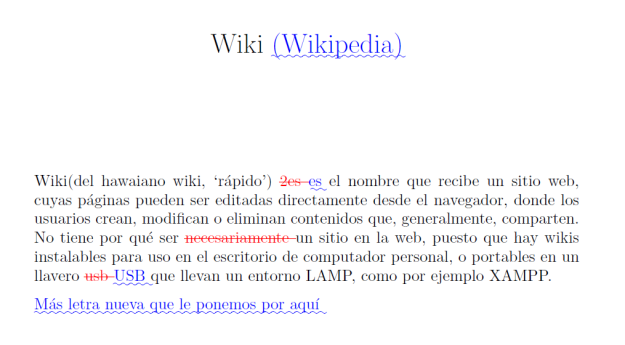
\includegraphics[width=\textwidth]{docs/Figuras/diff.png}
\caption{Marcando las diferencias}
\end{figure}

Tacha en rojo lo que hemos borrado y destaca en azul lo que hemos
añadido. Me parece especialmente útil para cuando estamos colaborando,
se ve de un vistazo cómo quedan los cambios.

Por cierto, si no queréis instalar nada también hay una
\href{https://3142.nl/latex-diff/}{versión online} en la que pegamos el
contenido de los archivos a comparar y nos aparece el archivo de
diferencias que podemos a su vez copiar y compilar.

\section{Exportar a LaTeX}

Este último apartado sobre las herramientas trata de exportar contenido
que tenemos en otros formatos a LaTeX. De esta manera conseguimos dos
cosas:

\begin{itemize}
\item
  Incluir con facilidad contenido creado en otros programas en LaTeX.
\item
  Ayudarnos a crear elementos que resultan complejos de llevar a cabo en
  LaTeX, como podrían ser las tablas y las portadas.
\end{itemize}

En el caso de las tablas se entrelazan ambas problemáticas, cuesta
escribir tablas en LaTeX y, además, muchas veces tenemos esas tablas en
otros formatos. Si nuestro problema es el primero, tenemos
\href{http://www.tablesgenerator.com/}{\emph{editores online}} con los
que crear la tabla de manera visual y exportarla a continuación. Si nos
pasan un poco de las dos cosas tenemos varias herramientas, la que más
he usado ha sido
\href{http://www.ctan.org/tex-archive/support/excel2latex/}{\emph{Excel2Latex}},
un \emph{plugin} para Excel que nos permite seleccionar y exportar una
tabla concreta en formato LaTeX, la verdad es que funciona bastante
bien. También hay una versión para OpenOffice,
\href{http://calc2latex.sourceforge.net/}{\emph{Calc2LaTeX}}, pero es
viejecita y no sé qué tal funciona, y tenemos
\href{https://github.com/TheChymera/matrix2latex}{\emph{Matrix2LaTeX}}
para Python y Matlab que no he usado.

Una herramienta similar es
\href{https://extensions.libreoffice.org/extensions/writer2latex-1}{\emph{Writer2LaTeX}}
que sirve para exportar de Libre Office Writer a LaTeX, no es la panacea
pero nos puede ayudar cuando tenemos que seguir cierta plantilla y solo
nos proporcionan un \emph{doc}, ¿os suena esto?

Sin duda el programa definitivo para las labores de conversión es
\href{http://pandoc.org/}{\emph{Pandoc}}, del que ya hemos hablado y que
trataremos largo y tendido dentro de poco. Con una terminal y una orden
muy sencilla transforma casi cualquier formato de texto a casi cualquier
otro:

\begin{lstlisting}[language=bash]
pandoc OPCIONES INPUT -o OUTPUT
\end{lstlisting}

\section{Resumen}

En este capítulo he mencionado diferentes herramientas útiles sin entrar
demasiado en detalle para que vosotros mismos investiguéis las que mejor
se adapten a vuestras necesidades. Hemos hablado de borradores, texto e
imágenes de prueba, plantillas, clases y paquetes, control de versiones
y sobre cómo exportar el contenido creado en otros programas a LaTeX.
Evidentemente, hay muchas más herramientas relacionadas con LaTeX ahí
fuera, estas son las que me han servido a mí en mi larga relación con
este lenguaje de marcado tan simpático.

\section{Referencias}

\href{https://tex.stackexchange.com/questions/49277/what-does-the-draft-mode-change}{\emph{What
does the draft mode change?} en TeXExchange}

\href{http://tug.ctan.org/info/dickimaw/dickimaw-minexample.pdf}{\emph{Creating
a LaTeX Minimal Example} (pdf)}

\href{https://www.ctan.org/pkg/lipsum}{El paquete \lstinline!lipsum!}

\href{https://www.ctan.org/pkg/blindtext}{El paquete
\lstinline!blindtext!}

\href{http://tex.stackexchange.com/questions/231738/example-images-in-latex\#231741}{\emph{Example
images in LaTeX?} en TexExchange}

\href{https://tex.stackexchange.com/questions/278817/creating-a-default-preamble}{\emph{Creating
a default preamble} en TeXExchange}

\href{https://docs.kde.org/stable4/en/extragear-office/kile/kile.pdf}{Manual
de Kile (pdf)}

\href{http://texstudio.sourceforge.net/manual/current/usermanual_en.html\#SECTION12aa}{Manual
de TexStudio}

\href{https://en.wikibooks.org/wiki/LaTeX/Creating_Packages}{\emph{LaTeX/Creating
Packages} en Wikibooks}

\href{http://www.latex-project.org/help/documentation/clsguide.pdf}{\emph{LaTeX
2$\varepsilon$ for class and package writers}}

\href{https://tex.stackexchange.com/questions/6560/best-practice-for-maintaining-change-history-in-tex}{\emph{Best
practice for maintaining change history in tex} en TeXExchange}

\href{https://robjhyndman.com/hyndsight/tracking-changes-in-latex-files/}{\emph{Tracking
changes in LaTeX files}}

\href{https://ondahostil.wordpress.com/2017/04/24/lo-que-he-aprendido-registro-de-cambios-en-un-documento-latex-con-git/}{\emph{Registro
de cambios en un documento LaTeX con git}}

\href{https://tex.stackexchange.com/questions/161/latex-packages-for-use-with-revision-control}{\emph{LaTeX
packages for use with revision control}}

\href{http://techshangrila.blogspot.com.es/2013/10/installing-latexdiff-of-windows.html}{\emph{Highlighting
the different between Latex Documents in Windows 7 using Latexdiff}}

\href{https://en.wikibooks.org/wiki/LaTeX/Collaborative_Writing_of_LaTeX_Documents}{\emph{LaTeX/Collaborative
Writing of LaTeX Documents} en Wikibooks}

\href{https://support.rstudio.com/hc/en-us/articles/200532257-Customizing-LaTeX-Options}{\emph{When
and why should I use \% !TEX TS-program and \% !TEX encoding?} en
TeXExchange}

\href{https://latexforhumans.wordpress.com/tag/calc2latex/}{\emph{Converting
a spreadsheet to LaTeX}}
